\section{Board Layer}
Après une configuration de la board réalisé avec \emph{STM32CubeMX} (détail
de la configuration dans le \emph{Guide ButtonsController}\footnotemark[1])
Dans la \emph{Board Layer}, la machine d'état du \emph{ButtonsController}
est implémentée.
\begin{figure}[H]
    \centering
    \includegraphics[width=0.45\textwidth]{Images/buttons/btnCtrl.PNG}
    \caption[Full UML]{State diagram du BoutonsController (provenant du \emph{Guide ButtonsController}\footnotemark[1])}
\end{figure}
\footnotetext[1]{\cite{lab_guide}}
Le fonctionnement de cette couche est simple : une interruption Hardware enclenche
le \emph{STATE\_DEBOUNCE}. Après 100 millisec, on retourne dans l'état d'attente,
et on contrôle l'état de tous les boutons. Ce temps d'attente permet de réaliser un
anti-rebond software.\newpage

\section{Middleware Layer}
Le \emph{Middleware} implémente la détection d'appui court ou long sur un bouton.
Elle reçoit les informations de la \emph{Board Layer} pour son fonctionnement, et
transmet les informations d'appui court ou long à la couche \emph{Application}
\subsection{Liaison avec la Board Layer}
La liaison avec la couche en dessous ce fait ainsi :
\begin{figure}[H]
    \centering
    \includegraphics[width=0.75\textwidth]{Images/buttons/mdw_layer.PNG}
    \caption[Full UML]{Diagramme de classe du mdw (provenant du \emph{Guide ButtonsController}\footnotemark[1])}
\end{figure}
\footnotetext[1]{\cite{lab_guide}}
Le \emph{ButtonEventsHandler} implémente l'interface \emph{ButtonsControllerCallbackProvider}
pour fournir la méthode \textbf{onButtonChanged} en méthode de callback.
La méthode de callback sera appelée par le \emph{ButtonsControllerCallbackCaller}.
Cela permet donc au \emph{ButtonsController} d'informer le \emph{ButtonEventsHandler}
d'un changement sur un bouton, sans aucune liaison direct entre les deux classes.
\newpage

\subsection{ButtonEventsHandler}
Le gestionnaire d'évenement boutons \emph{ButtonEventsHandler} fonctionne ainsi :
\begin{figure}[H]
    \centering
    \includegraphics[width=0.3\textwidth]{Images/buttons/btnEvHandler.PNG}
    \caption[Full UML]{Diagramme de classe du \emph{ButtonEventsHandler}
    (provenant du \emph{Guide ButtonsController}\footnotemark[1])}
\end{figure}
Lorsqu'il reçoit une information sur un bouton, il transmet un évenement
au \emph{ButtonStateSM} correspondant. Chaque \emph{ButtonStateSM} possède
une machine d'état interne :
\begin{figure}[H]
    \centering
    \includegraphics[width=0.75\textwidth]{Images/buttons/btnSM.PNG}
    \caption[Full UML]{Diagramme d'état d'un \emph{ButtonStateSM}
    (provenant du \emph{Guide ButtonsController}\footnotemark[1])}
\end{figure}
\footnotetext[1]{\cite{lab_guide}}
La machine d'état reçoit l'évenement \textbf{evButtonPressed}.
Une fois à l'état pressé, si le bouton est relaché avant 1 sec, elle notifie
le \emph{ButtonEventsHandler} d'un appui court, sinon d'un appui long.\newpage

\section{Application Layer}
\subsection{Liaison avec le Middleware}
\begin{figure}[H]
    \centering
    \includegraphics[width=0.75\textwidth]{Images/buttons/app_layer.PNG}
    \caption[Full UML]{Diagramme de classe de l'App (provenant du \emph{Guide ButtonsController}\footnotemark[1])}
\end{figure}
\footnotetext[1]{\cite{lab_guide}}
Pour permettre d'ajouter plusieurs module a la couche \emph{Application},
un patterne \emph{Subject - Observer} a été utilisé.
Le \emph{ButtonEventsHandler} possède une liste d'\emph{Observer}, a qui il
va notifier les appuis longs ou court. Les \emph{Observers} vont pouvoir
\textbf{subscribe} au \emph{Subjet} pour informer qu'ils souhaitent être notifié
des évenement boutons.
\subsection{Découplage complet du ButtonEventsLogger}
Pour découpler "totalement" le \emph{ButtonEventsLogger}, il a été demandé
d'en faire une machine d'état.
\begin{figure}[H]
    \centering
    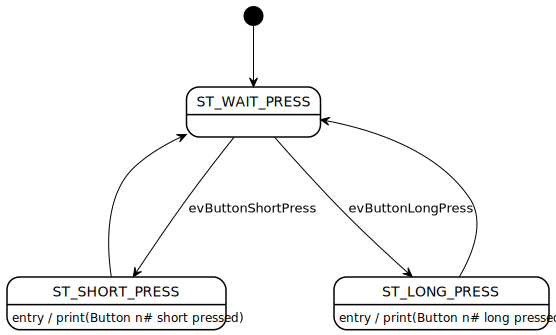
\includegraphics[width=0.6\textwidth]{Images/buttons/ButtonEventsLogger.png}
    \caption[Full UML]{Diagramme d'état du \emph{ButtonEventsLogger}}
\end{figure}\newpage

\subsection{ButtonEventsLedFlasher}
Le \emph{ButtonEventsLedFlasher} transmet les évenement \textbf{evButtonShortPress} et 
\textbf{evButtonLongPress} à des machines d'états \emph{LedStateSM} :
\begin{figure}[H]
    \centering
    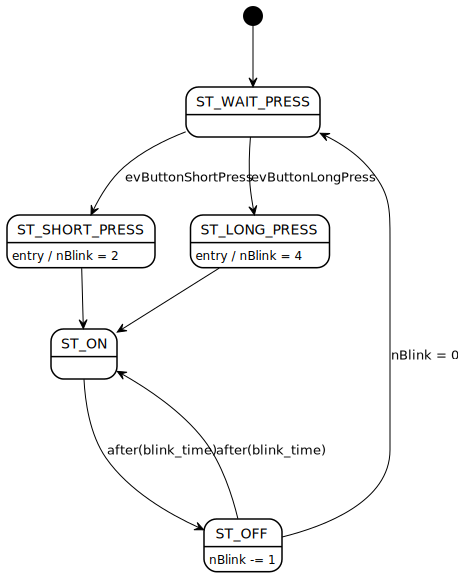
\includegraphics[width=0.5\textwidth]{Images/buttons/LedsStateSM.png}
    \caption[Full UML]{Diagramme d'état d'une \emph{LedStateSM}}
\end{figure}
Ces machines d'états appellent ensuite des méthode du \emph{LedsController} fournit
dans les modules de base.